\chapter{Incremental view synchronization}
\label{chap:transform}

Complex industrial toolchains used for the model-based design of safety-critical cyber-physical systems frequently depend on various models on different levels of abstraction where abstract models are derived by model transformations. The derived models are often \emph{views}, which aim to focus attention from a given \emph{viewpoint} such that details relevant to a specific group of stakeholders are retained~\citep{Bruneliere17survey}. The views contain information that is related to and coming from other models, which can also be themselves other views. Incremental small-step execution of model transformations aids in reducing the computations costs of view maintenance~\citep{Varro15styles}.

In this chapter we propose a means to assemble formal stochastic models from domain models by model transformation. The resulting analysis model is a \emph{view} of the engineering model from a \emph{reliability} or \emph{performability} viewpoint. The transformation should be \circled{1}~\emph{parametric} in the sense that the source metamodel, the transformation rules and the analysis model fragments that are instantiated may be specified by the user. In addition, stochastic Petri nets produced by the transformation should be \circled{2}~\emph{compatible with external analysis tools.} As a key to interpret analysis results of the derived stochastic models automatically, the transformation should ensure \circled{3}~\emph{end-to-end traceability} between source model elements and the quantitative aspects of the stochastic model. Lastly, to support efficient mapping of constantly changing design candidates in design-space exploration, the transformation should be \circled{4}~\emph{executed incrementally} driven by change notifications of the source model.

Existing transformation languages, such as \textabbr{ATL}~\citep{Jouault08atl}, \mixedabbr{QVT}r~\citep[Chapter~7]{OMG16qvt} or \textabbr{VIATRA} Views~\citep{Debreceni14viewmodel} can describe mappings between instances of arbitrary metamodels; therefore they satisfy the requirement of \circled{1}~user configurability. These language require the specification of the results of the transformation at the low level of individual model objects and links. While creating single objects at once is satisfactory for views that aim to create \emph{abstractions} of the source model, automatic derivation of stochastic models is closer to \emph{compilation}. The result of mapping even just one source element may have a complicated result, such as a collection of Petri net places, transitions and expressions trees describing quantitative aspects of the model. Hence we propose a transformation specification language tightly integrated with \textAbbr{RGSPN}s introduced in \cref{chap:rgspn} as an alternative to general-purpose transformation languages for stochastic model creation.

The left side of the transformation rules are graph patterns which select the parts of the source model to be mapped. On the right side, the transformation results are specified as \emph{\textabbr{RGSPN} modules}, which are \textAbbr{RGSPN} model fragments. The typing discipline from \vref{dfn:rgspn:well-typed} is extended to transformation rules to aid in catching bugs.

In current analysis tools, there is little support for reference symbols, variables and collections introduced in \textAbbr{RGSPN}s. To \circled{2}~ensure compatbility, a \emph{inlining} step is also incorporated into the transformation chain. The inlining \emph{concretizes} the \emph{abstract} \textabbr{RGSPN} constructed according to the user-provided view specification and yields a \emph{concrete} \textabbr{RGSPN}, that contains no references, collections or references to variables. Variable symbols are kept so that they can exported to the analysis tool as stochastic metrics to be computed or as queries to be answered. Matching of the queries to source model concepts is provided by \circled{3}~traceability relations that are maintained implicitly, i.e.~without additional user intervention.

The \circled{4}~incremental execution of the transformation is ensured by the use of an incremental graph query engine~\citep{Ujhelyi15incquery} and a reactive model transformation platform~\citep{Bergmann15viatra}. If a step in the transformation chain cannot be executed due to a malformed input model the effects of the transformation are \emph{delayed} until the issue is resolved. Upon delaying, an error marker is generated that is removed when the transformation can resume successfully.

After briefly reviewing related work we describe the proposed transformation chains, as well as its specification language and semantics. Then the instantiation of \textabbr{RGSPN} modules is discussed, finally followed by the details of the concretization transformation and its handling of inconsistencies by the means of delayed execution.

\section{Related work: view synchronization approaches}
\label{chap:transform:relwork}

Now we briefly review some approaches for synchronizing view models for engineering \textAbbr{DSL}s with a focus on approaches supporting incremental synchronization and the creation of complex formal modes.

Model transformations are a pervasive concept in model-driven engineering (\textabbr{MDE}) where they are employed to modify a model \emph{in place} or convert between different representations and abstraction levels of models by either creating a \emph{new target} model or \emph{updating} an existing one~\citep{Czarnecki06survey}. For transformations with separate source and targets, \emph{tracing} connects related source and target objects. The traceability model may be maintained \emph{manually} (\emph{explicitly}), or the transformation engine may provide \emph{automatic} (\emph{implicit}) traceability. \emph{Batch} execution re-evaluates the whole transformation when the source model changes to create a new version of the target. In contrast, \emph{target incrementality} (\emph{change propagation}) only performs necessary changes on the target model. \emph{Source incremental} transformations also attempt to minimize the re-examined portion of the source model, for example, by subscribing to change notifications.

\citet{Varro15styles} categorized the styles of change-driven model transformations as follows:
\begin{inparaenum}
\item Transformations with \emph{no incrementality} only execute in batch mode.
\item \emph{Dirty incrementality} marks target models or elements to be recomputed as dirty upon source changes and re-runs the transformation for the dirty portions.
\item \emph{Incrementality by traceability} relies of missing or dangling traceability links to determine the target elements that are created or removed.
\item \emph{Reactive source incrementality} triggers transformation rules by change notifications without relying on traceability links.
\end{inparaenum}

View transformations are specific models transformations that aim to create target models that describe the source from a specific viewpoint. \citet{Bruneliere17survey} has surveyed view transformation tools, including incremental approaches.

The \textabbr{ATL} transformation language is a domain-specific language for describing model-to-model transformations with implicit traceability~\citep{Jouault08atl}. Algorithms for trace-based incremental \textabbr{ATL} execution were proposed by \citet{Xiong07incremental}, as well as by \citet{Jouault10incremental}.

The Query-View-Transformation (\textabbr{QVT}) family of languages were also developed for describing model-to-model transformations~\citep{OMG16qvt}. The \emph{relation} \mixedabbr{QVT}r sublanguage is a declarative language for the correspondences between the source and target models with implicit traceability, which is compiled to the simple \emph{core} \mixedabbr{QVT}c sublanguage. The \emph{operational} \mixedabbr{QVT}o sublanguage provides imperative transformations. \citet{Song11incremental} proposed trace based incremental transformation for a subset of \mixedabbr{QVT}r suitable for deriving runtime models.

Triple grammars grammars (\textabbr{TGG}) can describe model transformations by employing and explicit trace model called the \emph{correspondence} model~\citep{Schurr94tgg}. Restrictions of \textAbbr{TGG}s~(view \textAbbr{TGG}s) have been proposed for incremental view synchronization~\citep{Jakob06nonmaterialized,Anjorin14materialized}. \citet{Greenyer11advanced} proposed extension for \textAbbr{TGG}s so that they could derive formal models from sequence diagram specifications. However, their approach does not support incremental execution.

The \textabbr{VIATRA} reactive model transformation platform provides a framework for change-driven model transformations with optional manual traceability~\citep{Bergmann15viatra}. \citet{Debreceni14viewmodel} proposed \textabbr{VIATRA} Views as a declarative, incremental view transformation engine built on incremental model queries~\citep{Ujhelyi15incquery} and \textabbr{VIATRA}.

\begin{figure}
  \centering
  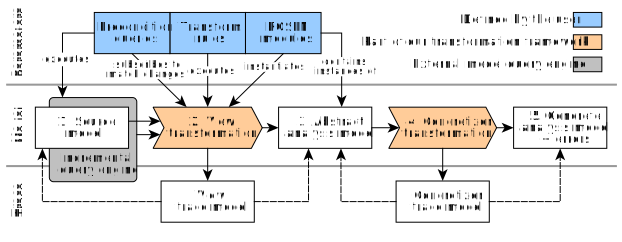
\includegraphics[scale=0.9]{figures/transformation_chain}
  \caption{Overview of the transformation chain.}
  \label{fig:transform:overview}
\end{figure}

\citet{Mosteller16semantics} proposed an approach to define semantics of domain-specific modeling languages by Petri nets in the Renew meta-modeling and transformation framework. A specialized modeling tool is generated based on a mapping from \textabbr{DSL} elements to Petri net fragments. The user can manipulate the concrete syntax of the \textabbr{DSL} while a Petri net is assembled from the fragments by the tool for analysis and code generation.

The ability to reference target objects created by different transformation rules is especially important in incremental transformation languages, because the developer of the transformations cannot rely on the order of rule executions. Hence transformation rules must be able to share target objects regardless their execution order.

In \textabbr{ATL} model elements generated by rules can be resolved at any time by the built-in \lit{resolveTemp} operation. In \mixedabbr{QVT}r relations between source and target elements can be joined by \lit{when} clauses. In \textAbbr{TGG}s target object sharing is implicitly present in the correspondence parts of the rule triples. \citet{Greenyer11advanced} introduced \emph{reusable patterns} to \textAbbr{TGG}s to further refine object sharing. \textabbr{VIATRA} Views support referencing objects produces by other rules with the \lit{@Lookup} annotation. In contrast, modular Petri nets~\citep{Kindler09modular} and thus our \textAbbr{RGSPN} fragments model importing symbols explicitly by reference symbols and reference assignments.


\section{Overview of the transformation engine}
\label{chap:transfrom:specify}

The transformation chain from engineering models to analyzable \textAbbr{RGSPN}s is shown in \vref{fig:transform:overview}. The architecture is divided into three parts: \begin{inparaenum}
\item the \emph{parameters} of the transformation, which constitute the transformation specification provided by the user,
\item the \emph{models} and model transformations participating in the chain and
\item the \emph{trace} models providing end-to-end traceability.
\end{inparaenum}

\subsection{Transformation specification}

The transformation description contains the \emph{precondition queries}, which are executed on an incremental model query engine. For each query match the \emph{transformation rules} specify which \emph{\textabbr{RGSPN}} module should be instantiated.

In addition, the user is able to reuse quantitative aspects of the engineering model in the analysis model and define new quantitative aspects to be evaluated as stochastic queries. These \emph{associated symbols}, along with their traceability information play roles similar to the parameters (prefixed with \enquote{\$}), stochastic metrics (\enquote{/}) and queries (\enquote{/\$}) introduced as an extension to \textabbr{UML} diagrams by \citet{Bernardi03building}.

Transformation rules can govern the mapping of numeric attributes from the domain model to the variable symbols of the \textabbr{RGSPN}. Attributes may be marked as parameters, which are retained as parameters symbols in \textabbr{RGSPN} and when the analysis model is exported to external solvers. Therefore the parameter mapping relates domain attributes to sensitivity analysis~\citep{Blake88sensitivity}, parametric solution of Markov chains~\citep{Hahn11parametric} and parameter synthesis \citep{Quatmann16mdp,Molnar17optimization}, letting users perform the aforementioned tasks directly on the domain model.

Moreover, \emph{derived} features may also be specified that associate \textabbr{RGSPN} symbols with domain model elements. In contrast with model query based approaches for the creation of derived features~\citep{Rath12derived} the domain model is not modified to incorporate the features. However, code generation and the \emph{extension methods} feature of \emph{Xtend}\footnoteurl{https://www.eclipse.org/xtend/} are utilized in \vref{sec:apply:environment} to emulate derived features syntactically in a general purpose programming language.

\subsection{Transformation chain}

As it is shown in \vref{fig:transform:overview} the construction of \textabbr{RGSPN} analysis models is realized as a \emph{chain} of two model transformations.

The precondition queries of transformation rules are ran on the 1.~\emph{source model} by an \emph{incremental query engine}. The 2.~\emph{view transformation} maintains a 3.~\emph{abstract analysis model} based on the query matches of the precondition queries and instantiates the \textabbr{RGSPN} modules according to the transformation rules. In addition, the associated symbols relating to the quantitative aspects of the source model elements are instantiated. A \emph{view trace model} links the elements and query matches of the source model to the symbols of the abstract \textabbr{RGSPN}.

The abstract \textabbr{RGSPN} contains reference symbols, variables and collections that are not directly exportable to analysis tools. Therefore the 4.~\emph{concretizer transformation} is needed to \emph{inline} these features and obtain a 5.~\emph{concrete analysis model}, which is an \textabbr{RGSPN} without advanced features. The concrete model can be exported as a \textabbr{GSPN} possibly parameter- and marking-dependent transition rates for analysis with external tools. Furthermore, the value expressions of the retained variable symbols, which refer to elements of the concrete model, can serve as stochastic metrics and queries to be analyzed.

If the abstract analysis model is inconsistent, e.g.~it contains unassigned references or circular references, concretization is delayed and \emph{error} markers are generated until the inconsistency is resolved. The \emph{concretizer trace model} links the abstract analysis model to the concrete one; moreover, it also allows the interpretation of error markers.

Both the concrete and abstract \textAbbr{RGSPN}s are fully materialized as instance models so that they can be freely inspected and exported. It is also possible to subscribe to change notification of either of the models, for example, to incorporate our transformation chain into a larger chain.

\subsection{End-to-end traceability}

Fully traversing the view and concretizer trace models allows the association of concrete \textabbr{RGSPN} symbols with source model elements. Thus when an external solver is interfaced with the transformation, it is sufficient to provide traceability between the concrete analysis model and the external solver so that the analysis results remain interpretable in the context of the source domain model.

\begin{figure}
  \centering
  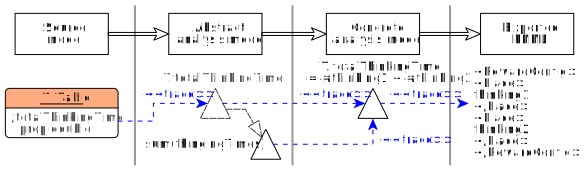
\includegraphics[scale=0.9]{figures/derived_feature_traceability}
  \caption{Traceability for associated symbols.}
  \label{fig:transform:derived}
\end{figure}

\begin{runningExample}
  \Vref{fig:transform:derived} shows the trace links for an \textabbr{RGSPN} symbol derived feature \lit{total\-Thinking\-Time} of the domain class \lit{Table}.

  The first trace link is the view trace model associates the domain object \lit{T} with the reference symbol \lit{T.total\-Thinking\-Time} in the abstract analysis model. A variable symbol is assigned to the reference.

  The concretization transformation resolves and inlines all references, therefore both trace links from the reference symbol and the concrete symbol in the concretization trace model point at the same variable symbol in the concrete analysis model. As result of the inlining, the aggregation operator in value expression of the variable is replaced with the sum of the member variables. In the example, these members are token count expressions \lit{\#thinking1} and \lit{\#thinking2}.

  If the concrete analysis model is exported to an external analysis tool, such as PetriDotNet~\citep{Voros17pdn}, the \textabbr{PNML} serializer may also output traceability information. In the example, the value expression of \lit{T.total\-Thinking\-Time} is turned into a reward configuration for PetriDotNet. The end-to-end trace links associate the exported reward configuration with the derived feature, hence the results of stochastic analysis can be interpreted in the context of the domain model and its derived features.
\end{runningExample}

\section{Transformation specification language}

We present the transformation specification language trough a running example. \Cref{tbl:transform:feature,tbl:transform:mapping} show an example transformation description for the dining philosophers domain. On the left graph patterns are displayed as subgraphs, while the \textabbr{RGSPN} modules on the right also use graphical concrete syntax. In the middle column, the textual concrete syntax of transformation descriptions is shown.

\subsection{Feature rules}

The first section of the transformation specification contains \emph{feature rules} that describe the associated symbols relating to the \emph{features} (\emph{attributes}) of the domain model elements. The feature rule section is introduced by the \lit{features} keyword. Each domain class may have a sub-section describing the mapping of its features.

By default, each \lit{int}, \lit{double} and \lit{boolean} attribute of a domain class is mapped to a \lit{const} variable symbol in the abstract \textabbr{RGSPN}. The value expression of the variable symbol is a literal that equals to the value of the domain attribute.

Users may override the attribute mapping of \lit{double} features by specifying \lit{param} mapping instead. Attributes marked as \lit{param} are turned into parameter symbols instead.

Lastly, feature rules may specify \texttt{derived} features. An \textabbr{RGSPN} reference symbol with the given type and name is created and is associated with the domain element.

\begin{table}%
  \caption{Feature rules for dining philosophers transformation specification.}%
  \label{tbl:transform:feature}
  \lstset{
    basicstyle={\ttfamily\small},
    columns=fixed,numbers=none,
    aboveskip=0pt,belowskip=-1.2\baselineskip,
    language=ecore2pn
  }%
  \centering
  \begin{tabular}{@{}>{\centering\arraybackslash}m{0.20\textwidth}@{}m{0.42\textwidth}@{}>{\centering\arraybackslash}m{0.38\textwidth}@{}}
    \toprule
    \multicolumn{1}{@{}c}{Domain class} & \multicolumn{1}{c}{Transformation rule} &
    \multicolumn{1}{c@{}}{Associated symbols} \\
    \midrule
    & \begin{lstlisting}
features {
\end{lstlisting} & \\
    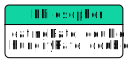
\includegraphics[scale=0.8]{figures/phil_class}& \begin{lstlisting}
  Philosopher {
    param eatingRate
  }
\end{lstlisting} &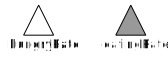
\includegraphics[scale=0.8]{figures/phil_features}\\
  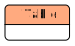
\includegraphics[scale=0.8]{figures/table_class}& \begin{lstlisting}
  Table {
    derived prop double
        ^totalThinkingTime^
  }
\end{lstlisting} &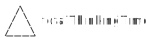
\includegraphics[scale=0.8]{figures/table_features}\\
  & \begin{lstlisting}
}
\end{lstlisting} &\\
    \bottomrule
  \end{tabular}
\end{table}

\begin{runningExample}
  The metamodel for the dining philosophers domain contains the classes \lit{Philosopher} and \lit{Table}. The two attributes of type \lit{double} of \lit{Philosopher} are \lit{eating\-Rate} and \lit{hungry\-Rate}, while \lit{Table} has no attributes.

  For \lit{Philosopher} the feature rule in \vref{tbl:transform:feature} marks the attribute \lit{eating\-Rate} as a parameter. Hence \lit{eating\-Rate} is mapped to the \textabbr{RGSPN} as a parameter symbol, while \lit{const} variable symbol is created for \lit{hungry\-Rate}.

  The \lit{Table} feature rule prescribes a derived feature \lit{total\-Thinking\-Time} of type \(\vartype{\lit{prop}}{\lit{double}}\). Hence a reference symbol with the same name and type is associated with \lit{Table} objects.
\end{runningExample}

\subsection{Mapping rules}

A \emph{mapping} rule associates a \emph{precondition} model query with a set of \emph{lookup declarations}, assignments and collections membership declarations, as well as optionally a \emph{postcondition} \textabbr{RGSPN} module. Thus the abstract analysis modules is weaved from \textabbr{RGSPN} module instances and the edges added between them by the mappings.

For every tuple of match arguments in the match set of the precondition query instances of the assignments, collections memberships and the \textabbr{RGSPN} module are added to the abstract analysis model. The instantiation of modules is perfomed by copying their contents to the abstract analysis model after renaming their symbols to avoid collisions. The match argument tuple serves as the source of traceability links to the instantiated objects.

After the keyword \lit{mapping} the precondition graph pattern is named, followed by its list of parameters. The associated symbols of match arguments are accessible in the body of the mapping rule by mentioning the name of the match argument, followed by the dot operator and the name of the associated symbol.

The name of the \textabbr{RGSPN} module to instantiate and a \emph{local name} for the module instance may be specified after the \lit{=>} operator. If the module instantiation clause is present symbols inside the module instance can be referred to using the local name of the instance and the dot operator similarly to associated symbol references.

\subsubsection{Lookup declarations}

The view trace model can be traversed during the view transformation by \emph{lookup declarations}, analogously to the \texttt{@Lookup} annotation introduced by \citet{Debreceni14viewmodel} for the traversal of traceability relations in view maintenance. Introduced by the keywords \lit{lookup} they name a precondition pattern and provide a list of match arguments. The match arguments must be a subset of the parameters of the containing mapping rule and a pattern match of the specified pattern must exist.

After the operator \lit{=>} a local name may be given to the module instance created by the lookup up mapping rule. Hence it is possible to refer to symbols instantiated by other mapping rules in order to connect them with the rest of the analysis model. The execution of the view transformation, which is described in \vref{chap:transform:view}, ensures that the modules can be instantiated in any order and allows cyclic lookups between mapping rules.

\subsubsection{Edge declarations}

Edges between different \textabbr{RGSPN} module instances and symbols associated with domain objects are also supported. The \lit{:=} and \lit{+=} operators may add reference assignments and collection membership edges, respectively. Typing rules in \vref{dfn:rgspn:well-typed} are checked in mapping rules as well as in \textabbr{RGSPN} modules. Thus the abstract \textabbr{RGSPN} output by the view transformation is ensured to be well-typed.

\begin{table}%
  \caption{Mapping rules for dining philosophers transformation specification.}%
  \label{tbl:transform:mapping}
  \lstset{
    basicstyle={\ttfamily\small},
    columns=fixed,numbers=none,
    aboveskip=0pt,belowskip=-1.2\baselineskip,
    language=ecore2pn
  }%
  \centering
  \begin{tabular}{@{}>{\centering\arraybackslash}m{0.20\textwidth}@{}m{0.42\textwidth}@{}>{\centering\arraybackslash}m{0.38\textwidth}@{}}
    \toprule
    \multicolumn{1}{@{}c}{Precondition} & \multicolumn{1}{c}{Transformation rule} &
    \multicolumn{1}{c@{}}{\textabbr{RGSPN} module} \\
    \midrule
    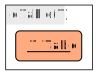
\includegraphics[scale=0.8]{figures/q_table_pattern}& \begin{lstlisting}
mapping qTable(T)
    => TableMod TM {
  T.^totalThinkingTime^
      := TM.totalThinkingTime
}
\end{lstlisting} &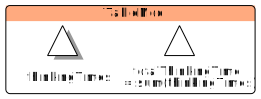
\includegraphics[scale=0.8]{figures/table_module}\\[-0.2ex]
  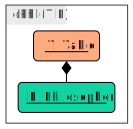
\includegraphics[scale=0.8]{figures/q_phil_pattern}& \begin{lstlisting}
mapping qPhil(T, P)
    => PhilMod PM {
  lookup qTable(T) => TM
  PM.^hungryRate^ := P.hungryRate
  PM.^eatingRate^ := P.eatingRate
  TM.^thinkingTimes^
      += PM.thinkingTime
}
\end{lstlisting} &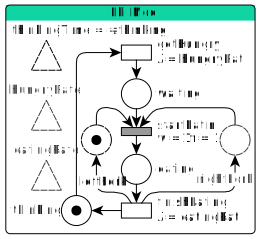
\includegraphics[scale=0.8]{figures/phil_module}\\[-2ex]
  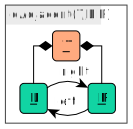
\includegraphics[scale=0.8]{figures/q_adjacent_pattern}& \begin{lstlisting}
mapping qAdjacent(T, L, R) {
  lookup qPhil(T, L) => PM1
  lookup qPhil(T, R) => PM2
  PM2.^leftFork^ := PM1.rightFork
}
\end{lstlisting} &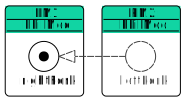
\includegraphics[scale=0.8]{figures/adjacent_phils_module}\\
    \bottomrule
  \end{tabular}
\end{table}

\begin{runningExample}
  In \vref{tbl:transform:mapping} three mapping rules are given for the dining philosophers domain. The feature rules in \vref{tbl:transform:feature} are assumed for the mappings.

  The pattern \lit{qTable} matches for all instances \lit{T} of the class \lit{Table}. An instance of the module \lit{TableMod} is created with the local name \lit{TM}. The symbol \lit{total\-Thinking\-Time} of \lit{TM} is assigned to the derived symbol with the same name of the domain object \lit{T}.

  The pattern \lit{qPhil} matches each philosopher \lit{P} sitting around a table \lit{T}. The corresponding mapping instantiates \lit{PhilMod} with the local name \lit{PM}. The table \lit{T} is included in the match parameter list such that the module \lit{TM} created by the mapping \lit{qTable} for \lit{T} can be looked up. The references \lit{hungry\-Rate} and \lit{eating\-Rate} inside \lit{PM} are assigned to the symbols constructed from the attributes of \lit{P}. The variable symbol \lit{thinking\-Time} of \lit{PM} is added to the collection \lit{thinking\-Times} of \lit{PM}.

  The interaction between the instances of \lit{TableMod} and \lit{PhilMod} showcases the advantages of collection symbols in \textAbbr{RGSPN}. The individual performance measures \lit{thinking\-Time} of philosophers are added to a collection, such that the aggregate performance measure \lit{total\-Thinking\-Time} can be computed.

  Lastly, \lit{qAdjacent} find philosophers \lit{L} and \lit{R} sitting next to each other around the table \lit{T}. While the corresponding mapping has no \textabbr{RGSPN} module to instantiate, it looks up the modules instances \lit{PM1} and \lit{PM2}, respectively. The reference to the left fork of the right philosopher is assigned to the right for of the left philosopher, which completes the dining philosophers model.
\end{runningExample}

\section{Generic view transformation to stochastic Petri nets}
\label{chap:transform:view}

The first transformation in our transformation chain is the view transformation that derives abstract \textabbr{RGSPN} analysis models from engineering model. Its four main objectives are
\begin{itemize*}
\item the instantiation of associated symbols for domain objects,
\item the instantiation of \textabbr{RGSPN} modules for mapping rule precondition matches,
\item the instantiation of additional assignment and collection membership edges according to lookup specifications and
\item the synchronization of the value expressions of associated attribute symbols with the values of domain attributes.
\end{itemize*}

The creation and removel of associated symbols, as well as \textabbr{RGSPN} modules and edges follows the strategy for incremental view maintenance by graph queries proposed by \citet{Debreceni14viewmodel}. Analysis model elements are created for precondition pattern matches with missing traceability links, while analysis model elements with dangling traceability links are deleted. Hence the style of instantiation is small-step \emph{incrementality by traceability}~\citep{Varro15styles}. The trace model is \emph{implicit}, i.e.~users do not need to define a metamodel for traceability links themselves. The transformation engine maintains the view trace model automatically instead.

Edges defined inside mapping rules are only instantiated when there is a traceability link for the abstract \textabbr{RGSPN} symbols on both ends of the edge and the precondition of the mapping rule matches. To this end a \emph{connection} graph pattern is generated which incorporates the precondition pattern and  also matches the traceability links for the looked up \textabbr{RGSPN} modules and associated symbols of the mapping rule. By evaluating the generated pattern over the source model and the view trace model jointly the set of edges that can be added to the abstract analysis model are determined. Dedicated traceability links are also added between the matches of the generated patterns and the inserted edges; therefore the edges can be removed when their corresponding match of the connection pattern disappears and the traceability link becomes dangling.

\begin{runningExample}
  The connection pattern generated from the mapping rule \lit{qTable} in \vref{tbl:transform:mapping} is \(\lit{qTable}^*(x) = \lit{qTable}(x) \land (\exists \ell_1 .\)\rel{mod\-ule\-In\-stance\-Trace}\((\lit{qTable}, \ltup x \rtup, \ell_1)) \land (\exists \ell_2 .\)\rel{as\-so\-ci\-a\-ted\-Sym\-bol\-Trace}\((x, \ell_2))\), where \rel{mod\-ule\-In\-stance\-Trace}\((\phi, t, \ell)\) indicates that \(\ell\) is the traceability link for the \textabbr{RGSPN} module instance created by the mapping rule with precondition \(\phi\) for the pattern match tuple \(t\) and \rel{as\-so\-ci\-a\-ted\-Sym\-bol\-Trace}\((x, \ell)\) indicates that \(\ell\) is the traceability link for the symbols associated with the source object \(x\). Likewise we have \(\lit{qPhil}^*(x, y) = \lit{qPhil}(x, y) \land (\exists \ell_1 .\)\rel{mod\-ule\-In\-stance\-Trace}\((\lit{qPhil}, \ltup x, y \rtup, \ell_1)) \land (\exists \ell_2 .\)\rel{as\-so\-ci\-a\-ted\-Sym\-bol\-Trace}\((y, \ell_2)) \land (\exists \ell_3 .\)\rel{mod\-ule\-In\-stance\-Trace}\((\lit{qTable}, \ltup x \rtup, \ell_3))\) and \(\lit{qAdjacent}^*(x, y, z) = \lit{qAdjacent}(x, y, z) \land (\exists \ell_1 .\)\rel{mod\-ule\-In\-stance\-Trace}\((\lit{qPhil}, \ltup x, y \rtup, \ell_1)) \land (\exists \ell_2 .\)\rel{mod\-ule\-In\-stance\-Trace}\((\lit{qPhil}, \ltup x, z \rtup, \ell_2))\).
\end{runningExample}

Symbols associated with numerical attributes of domain objects are synchronized with the values of the attributes. The transformation engine subscribes to change notifications from the source model and updates values of the symbols associated with the changed object. Hence the attribute synchronization is \emph{reactive source incremental}.

\begin{figure}
  \centering
  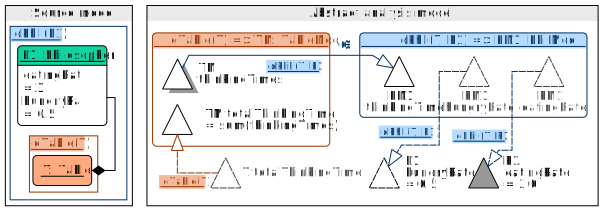
\includegraphics[scale=0.9]{figures/view_transformation_example_initial} 
  \caption{Initial setup for the example view transformation.}
  \label{fig:transform:view-1}
\end{figure}

\begin{figure}
  \centering
  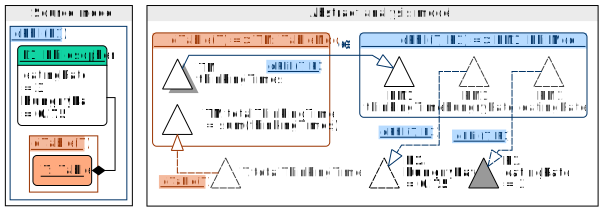
\includegraphics[scale=0.9]{figures/view_transformation_example_2}
  \caption{State of the example view transformation after modifying \lit{P1.eatingRate}.}
  \label{fig:transform:view-2}
\end{figure}

\begin{figure}
  \centering
  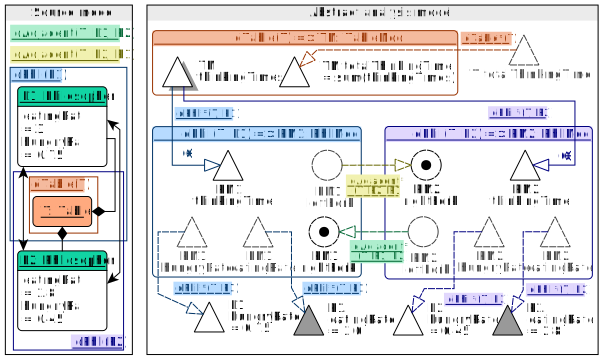
\includegraphics[scale=0.9]{figures/view_transformation_example}
  \caption{State of the example view transformation after adding a new philosopher \lit{P2}.}
  \label{fig:transform:view-3}
\end{figure}

\begin{runningExample}
  \Cref{fig:transform:view-1,fig:transform:view-2,fig:transform:view-3} show an example transformation of a dining philosophers domain model according to the feature rules in \vref{tbl:transform:feature} and the mapping rules in \vref{tbl:transform:mapping}. Symbols inside module instances with no adjacent edges between modules were suppressed for clarity. Trace links are indicated by writing the names of the linked pattern matches in the analysis model, as well as the coloring of pattern matches and model elements.

  The initial model in \vref{fig:transform:view-1} contains a \lit{Table} \lit{T} and a \lit{Philosopher} \lit{P1}. The precondition query \lit{qTable} has a single match \(\ltup \lit{T} \rtup\) and \lit{qPhil} has a single match \(\ltup \lit{T}, \lit{P1} \rtup\).

  The associated symbols \lit{P1.eatingRate} and \lit{P1.hungryRate} were created for \lit{P1}. The derived feature symbol \lit{T.totalThinkingTime} is associated with \lit{T}. Module instances \lit{TM} of \lit{TableMod} and \lit{PM1} of \lit{PhilMod} were also added to the abstract analysis model for the precondition matches \(\lit{qTable}\ltup \lit{T} \rtup\) and \(\lit{qPhil}\ltup \lit{T}, \lit{P1} \rtup\), respectively. The connection patterns \(\lit{qTable}^*\) generated from the \lit{qTable} mapping rule and \(\lit{qPhil}^*\) generated from the \lit{qPhil} mapping rule govern the insertion of \textabbr{RGSPN} edges between modules. The connection match \(\lit{qTable}^*\ltup \lit{T} \rtup\) assigns the variable \lit{TM.totalThinkingTime} to the derived reference \lit{T.totalThinkingTime}. In addition, \(\lit{qPhil}^*\ltup \lit{T}, \lit{P1} \rtup\) adds \lit{PM1.thinkingTime} to the collection \lit{TM.thinkingTimes} and assigns the features symbols associated with \lit{T} to the respective reference symbols in the module \lit{PM1} such that they can be mentioned in the expressions inside the implementation of \lit{PhilMod}.

  In \vref{fig:transform:view-2} the attribute \lit{hungryRate} of \lit{P1} was changed. Therefore the transformation synchronized the literal in the value expression of the feature symbol \lit{P1.hungryRate} in the abstract analysis model.

  In \vref{fig:transform:view-3} a new \lit{Philosopher} \lit{P2} was created, which sits both on the left and right of \lit{P1} around the circular table \lit{T}. New precondition matches \(\lit{qPhil}\ltup \lit{T}, \lit{P} \rtup\), \(\lit{qAdjacent}\ltup \lit{T}, \lit{P1}, \lit{P2} \rtup\) and \(\lit{qAdjacent}\ltup \lit{T}, \lit{P2}, \lit{P1} \rtup\) appeared, which lead to the instantiation of a new \lit{PhilMod} \lit{PM2}. The symbols inside the \lit{PM2} are connected to the rest of the analysis model with edges due to the connection match \(\lit{qPhil}^*\ltup \lit{T}, \lit{P} \rtup\). Furthermore, matches \(\lit{qAdjacent}^*\ltup \lit{T}, \lit{P1}, \lit{P2} \rtup\) and \(\lit{qAdjacent}^*\ltup \lit{T}, \lit{P2}, \lit{P1} \rtup\) of the connection query generated from the mapping rule \lit{qAdjacent} caused the assignments of \lit{PM1.leftFork} to \lit{PM2.rightFork} and \lit{PM2.leftFork} to \lit{PM2.rightFork}.

  Because analysis model elements with dangling trace links are removed the deletion of \lit{P2} from the source model would cause the view transformation to restore the analysis model to the state shown in \cref{fig:transform:view-2}.
\end{runningExample}

\section{Stochastic Petri net concretization}
\label{chap:transform:concretizer}

The second step in our transformation chain is the concretization with derives a \textabbr{RGSPN} containing only concrete symbols from the abstract analysis model. The resulting concrete analysis model can be readily exported as a parametric \textabbr{GSPN} to external solvers. In addition, variable symbols are preserved in the concrete analysis model so that they can serve as stochastic metrics and queries to be evaluated.

The three main responsibilities of the concretization transformation are
\begin{itemize*}
\item the copying of concrete place, transition, variable and parameter symbols from the abstract analysis model to the concrete analysis model,
\item the resolution of reference symbols and
\item the inlining of the variables and collection aggregations into \textabbr{RGSPN} expressions.
\end{itemize*}

The execution of the the aforementioned transformations may be prevented by errors and inconsistencies of the abstract analysis model. Inconsistency may be caused by a reference symbol having no resolution to a concrete symbol, reference resolution leading to parallel arcs or cyclic dependencies of expression. Robust inconsistency handling is especially important in change-driven incremental transformation chains, as a sequence of modifications of the source model may induce inconsistency in the abstract analysis model during execution even if the abstract analysis model becomes consistent at the end of the sequence. Our handling delays parts of the concretization until the inconsistency is resolved, while an error marker is generated to alert the user. The list of error markers can be checked at the end of source model modification sequences to ensure that the transformation chain fully synchronized the analysis models without hampering the execution of individual modification operations in the sequence.

\begin{figure}[p]%
  \begin{minipage}[t]{0.5\textwidth}
    \centering
    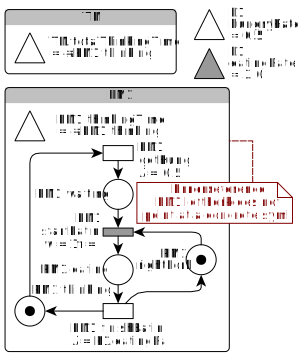
\includegraphics[scale=0.9]{figures/concrete_rgspn_example_initial}
    \caption{\protect\RaggedRight Concretization of the initial \textabbr{RGSPN} from \vref{fig:transform:view-1}.}
    \label{fig:transform:concrete-1}
  \end{minipage}%
  \begin{minipage}[t]{0.5\textwidth}
    \centering
    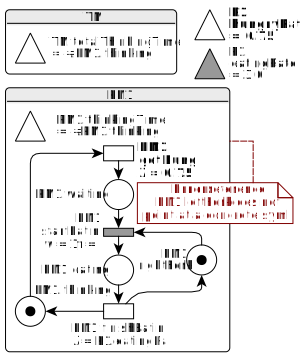
\includegraphics[scale=0.9]{figures/concrete_rgspn_example_2}
    \caption{\protect\RaggedRight Concretization of the \textabbr{RGSPN} from \vref{fig:transform:view-2} after changing \lit{P1.eatingRate}.}
    \label{fig:transform:concrete-2}
  \end{minipage}%
\end{figure}

\begin{figure}[p]
  \centering
  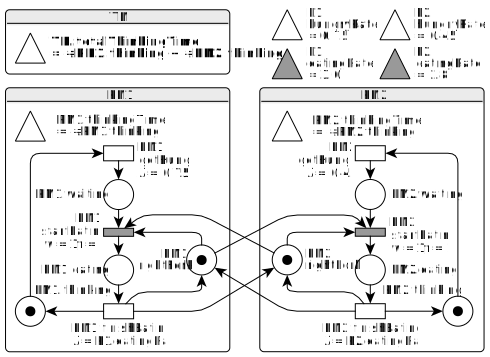
\includegraphics[scale=0.9]{figures/concrete_rgspn_example}
  \caption{Concretization of the \textabbr{RGSPN} from \vref{fig:transform:view-3}.}
  \label{fig:transform:concrete-3}
\end{figure}

\begin{runningExample}
  \Vref{fig:transform:concrete-1,fig:transform:concrete-2,fig:transform:concrete-3} show the concretizations of the abstract analysis models from \vref{fig:transform:view-1,fig:transform:view-2,fig:transform:view-3}. Traceability links are indicated by identical names of symbols in the abstract and concrete analysis models.

  \Vref{fig:transform:concrete-1} shows the initial concrete analysis model. Reference and collections symbols have been eliminated from the model. The mentioned reference symbol \lit{PM1.eatingRate} in  \(\lambda(\)\lit{PM1.finishEating}\()\) was replaced with the parameter symbol \lit{P1.eatingRate} by reference resolution. The value of the variable symbol \lit{P1.hugryRate} was inlined into \(\lambda(\)\lit{PM1.getHungry}\()\). The aggregation expression in \lit{TM.totalThinkingTime} was expanded into \lit{\#PM1.thinking}.

  All expressions in the conrete model are \enquote{flat}, i.e.~they contain no mentions of variables or collection aggregations. The only non-constant expressions are direct parameter and marking dependencies. While variable symbols are not mentioned in expressions of the Petri net, they remain in the model so that they can be exported as metrics and queries to external analysis tools.

  In \vref{fig:transform:view-1} the referenced \lit{PM1.leftFork} in the abstract analysis model did not point at any (concrete) symbol. Therefore the reference could not be resolved in \vref{fig:transform:concrete-1}. Creation of the arcs between \lit{PM1.startEating}, \lit{PM1.finishEating} and \lit{PM1.leftFork} in the concrete analysis model is \emph{delayed}. An error marker is generated indicating that the concretization was not fully completed.

  In \vref{fig:transform:view-2} the modification of the \lit{eatingRate} of \lit{P1} is propagated to the concrete \textabbr{RGSPN}. In contrast with \vref{fig:transform:view-2} not only the value expression of the variable symbol \lit{P1.eatingRate} is synchronized but also \(\lambda(\)\lit{PM1.finishEating}\()\) is updated. Because the reference \lit{PM1.leftFork} is still unresolved the error marker is preserved; however, the rest of the transformation could be executed.

  The addition of the \lit{Philosopher} \lit{P2} lead to a new \lit{PhilMod} instance \lit{PM2} in \vref{fig:transform:view-3}, which was copied into \vref{fig:transform:concrete-3}. Due to the reference resolutions~(see \vref{dfn:rgspn:resolution}) \lit{PM1.leftFork} \(\leadsto\) \lit{PM2.rightFork} and \lit{PM2.leftFork} \(\leadsto\) \lit{PM1.rightFork} all symbols and arcs could be concretized successfully. In the concrete \textabbr{RGSPN} the \lit{rightFork} symbols stand for the \lit{leftFork} symbols of the abstract \textabbr{RGSPN}. Moreover, the value expression of \lit{TM.totalThinkingTime} was update to accommodate the new element \lit{PM2.thinkingTime} \(=\) \lit{\#PM2.thinking} of the aggregated collection \lit{TM.thinkingTimes} in the abstract analysis model.
\end{runningExample}

\subsection{Transformation execution}
\label{sec:transform:execution}

The copying of place, transition, variable and parameter symbols is performed in a \emph{trace incremental} style, similarly to the instantiation of the abstract analysis model. The symbol in the abstract analysis model is connected to its \emph{image} in the concrete analysis model with a traceability link.

Resolution of references during copying is also trace incremental. To copy Petri net arcs \(s_1 \overset{e}{\inarc} s_2\) (or \(s_1 \overset{e}{\outarc} s_2\), \(s_1 \overset{e}{\inharc} s_2\), respectively) the symbols at both ends of the arc are resolved to concrete places and transitions according to \vref{dfn:rgspn:resolution} first, such that we have \(s_1 \leadsto p\) and \(s_2 \leadsto t\) for some transition \(t\) and place \(p\). Since \(p\) and \(t\) are located in the abstract analysis model, traceability links must be traversed to locate their images \(p'\) and \(t'\) in the concrete analysis model. Then the arc of the form \(p' \overset{e}{\inarc} t'\) can be added to the concrete analysis model and connected to \(s_1 \overset{e}{\inarc} s_2\) with a traceability link. The concretized arc is removed when any of its traceability links become dangling. 

In contrast, the inlining of expressions is not trace incremental, as the value of an expression may change even if no objects are added or removed in the abstract analysis model. A purely notification driven approach is also unsuitable, as an abstract analysis model change requires updating not only the image of the affected symbol in the concrete analysis model, but also the images of any expressions referring to the symbol, possibly through a chain of references or collection aggregations. A \emph{dirty incrementality} is employed instead, where symbols depending on changed source model elements are marked as dirty when the change notification is received. After the rest of the transformation rules have been processed the \emph{cleanup} rule is fired, which re-evaluates any expressions connected to dirty symbols without unnecessary duplication of computations.

\subsection{Expression dependencies}

In this section we describe the algorithm used for dirty marking and re-evaluation of expressions. The algorithm works on the level of symbols and arcs and re-evaluates any expressions connected to a symbol when cleaning up dirty marks. Although expression-level granularity could prevent event more re-evaluations compared to symbol-level dirty marking, in our evaluation \vref{sec:apply:eval} we found the scalability of the current approach acceptable.

Re-evaluation of the image of an expression may be required
\begin{itemize*}
\item when the value of a variable mentioned directly in the expression or indirectly through variable, references and collection aggregations changes,
\item when a reference assignment \(r \assign s\) of a directly or indirectly mentioned reference symbol \(r\) is created or removed,
\item when a collection membership edge \(c \member s\) of a directly or indirectly mentioned collection symbol \(c\) is created or removed.
\end{itemize*}

We formalize these notion as follows by mutually recursively defining the \(\rel{support}\colon \Sigma \cup \Expr_\Sigma \cup ({\inarc}) \cup ({\outarc}) \cup ({\inharc}) \to 2^\Sigma\) of expressions, symbols and arcs of an \textabbr{RGSPN} over the signature signature \(\Sigma\), as well as \emph{touching} of symbols:

\begin{dfn}
  The \emph{support} of an expression is the union of the supports of the symbols mentioned directly,
  \begin{equation}
    \rel{support}(e) = \quad\bigcup_{\hsmash{\text{\(s\) is mentioned in \(e\)}}}\quad \rel{support}(e) \text.
  \end{equation}
  
  The \emph{support} of a symbol contains itself, the supports of any expressions associated with the symbol, its pointed symbols and its collection members,
  \begin{multline}
    \rel{support}(s) = \{s\} \cup \rel{support}(m_0(s)) \cup \rel{support}(\lambda(s)) \cup \rel{support}(w(s))\\\cup \rel{support}(\pi(s)) \cup \rel{support}(\rel{value}(s)) \cup \bigcup_{s \assign s'} \rel{support}(s') \cup \bigcup_{s \member s'} \rel{support}(s')
  \end{multline}
  where \(P, T_T, T_i, V, \Par, R, C\) are the sets of places, timed transitions, immediate transitions, variables, parameters, references as collections of \(\Sigma\) according to \vref{dfn:rgspn:rgspn}.

  The \emph{support} of an arc \(\ltup p, e, t\rtup \in ({\inarc}) \cup ({\outarc}) \cup ({\inharc})\) is the support of its inscription,
  \begin{equation}
    \rel{support}(\ltup p, e, t \rtup) = \rel{support}(e) \text.
  \end{equation}

  The \(\rel{cone}\colon \Sigma \to 2^{\Sigma \cup (\inarc) \cup (\outarc) \cup (\inharc)}\) of a symbol is the set of symbols and arcs that contain it in their supports, which is the set of \textabbr{RGSPN} elements the symbol can affect,
  \begin{equation}
    \rel{cone}(s) = \{x \in \Sigma \cup (\inarc) \cup (\outarc) \cup (\inharc) \mid s \in \rel{support}(x)\} \text.
  \end{equation}
\end{dfn}

\begin{example}
  In \vref{fig:transform:view-3} the \rel{support} of \lit{T.to\-tal\-Think\-ing\-Time} is \(\{\)\lit{T.to\-tal\-Think\-ing\-Time}, \lit{TM.to\-tal\-Think\-ing\-Time}, \lit{TM.think\-ing\-Times}, \lit{PM1.think\-ing\-Time}, \lit{PM1.think\-ing}, \lit{PM2.think\-ing\-Time}, \lit{PM2.think\-ing}\(\}\). The \rel{cone} of \lit{P1.hung\-ry\-Rate} is \(\{\)\lit{P1.hung\-ry\-Rate, PM1.hung\-ry\-Rate, PM1.get\-Hung\-ry}\(\}\).
\end{example}

Note that \(r \assign^* s\) (and thus \(r \leadsto s\)) implies \(s \in \rel{support}(r)\) and \(r \in \rel{cone}(s)\).

\begin{dfn}
  A change of the abstract analysis model \emph{touches} a symbol \(s\) if
  \begin{compactitem}
  \item it changes the value of \(m_0(s)\), \(\lambda(s)\), \(w(s)\), \(\pi(s)\) of \(\rel{value}(s)\),
  \item it creates or removes an assignment edge of the form \(s \assign s'\),
  \item it creates or removes a collection membership edge of the form \(s \member s'\).
  \end{compactitem}
\end{dfn}

\begin{example}
  Changing \lit{P1.hung\-ry\-Rate} in \vref{fig:transform:view-2} touched \lit{P1.hung\-ry\-Rate}, because \(\lit{value}(\)\lit{P1.hung\-ry\-Rate}\()\) was modified. Adding a new philosopher \lit{P2} and its \textabbr{RGSPN} module \lit{PM2} in \vref{fig:transform:view-3} touched \lit{TM.think\-ing\-Times}, because the membership edge \lit{TM.think\-ing\-Times} \(\member\) \lit{PM2.think\-ing\-Time} was added.
\end{example}

When a change is to be propagated from the abstract analysis model to the conrete \textabbr{RGSPN}, the cones of any touched symbols are inspected. The images of symbols and arcs in the touched cones (if any) are marked as dirty in the concrete \textabbr{RGSPN}. Moreover, any symbol copied from the abstract analysis model starts as dirty. Dirtyness is tracked in the concretizer trace model.

After synchronizing any other change, such as the copying of concrete symbols and the removal of symbols with dangling traceability edges, the cleanup of dirty symbols and arcs proceeds. Symbols are cleaned up in the order of their dependencies. Lastly, dirty arcs are cleaned up by re-evaluating their inscriptions.

\begin{dfn}
  A symbol \(s_1'\) of the concrete analysis model \emph{precedes} \(s_2'\), written as \(s_1' \preceq s_2'\) if \(s_1'\) and \(s_2'\) are the images of \(s_1\) and \(s_2\) from the abstract analysis model, respectively, and \(s_1 \in \rel{support}(s_2)\).
\end{dfn}

Symbols \(s_1\) and \(s_2\) such that \(s_1 \neq s_2\), but both \(s_1 \in \rel{support}(s_2)\) and \(s_2 \in \rel{support}(s_1)\) constitute a \emph{circular dependency}, which will be identified as a source of inconsistency of the abstract analysis model in \vref{ssec:transform:inconsistent}. If there are no cicrular dependencies \(\preceq\) forms a partial order over the symbols of the concrete \textabbr{RGSPN}.

Symbol cleanup processes dirty symbols in nondecreasing order according to \(\preceq\). Each expression associated with a symbol is re-evaluated by inlining the values of mentioned variables, unfolding collection aggregations, as well as replacing mentioned places and parameter symbols by their images. These operations produce expressions equivalent to the originals according to the semantics described in \vref{ssec:rgspn:semantics}.

As the symbols are ordered by their dependencies upon traversal, there is no need to recursively process the value expressions of mentioned variable symbols. The variable symbol was already processed, because any mentioned variable is in the support of the expression; hence the image of the variable already has a re-evaluated value expression that was simplified as much as possible. Moreover, basic constant propagation arithmetic is performed if the result of evaluation is a Boolean or numerical constant.

After processing all the dirty symbols the inscriptions of dirty arcs are similarly re-evaluated. Because variables cannot depend on arc inscriptions the dependency order is not violated and variables can be inlined as above.

The concretizer transformation is aided by incremental model queries over the abstract \textabbr{RGSPN} and the concretizer trace model. The reflexive transitive closure of the assignment relation \(\assign^*\), the reference resolution relation \(\leadsto\) and supports of symbols in the abstract analysis model, as well as the dependency order \(\preceq\) on the concrete analysis model is maintained by incremental transitive closure computation~\citep{Bergmann12incscc}.

\begin{remark}
  Petri net \emph{slicing}~\citepeg{Llorens17slicing} uses tools closely related to our dependency tracking mechanism to extracts parts of a Petri net influencing the satisfaction of a property. Slicing could be incorporated in the future into the concretization transformation to avoid copying symbols to the concrete analysis model that are irrelevant to the (stochastic) properties of interest. Alternatively, the external analysis tools can slice their input Petri nets to reduce computational burden.
\end{remark}

\subsection{Handling of inconsistencies}
\label{ssec:transform:inconsistent}

Inconsistencies in the abstract \textabbr{RGSPN} analysis model refer to constraint violations that prevent the model from being concretized. While type checking for \textAbbr{RGSPN}s as defined in \vref{dfn:rgspn:well-typed} can prevent some problems at design time, other violations arise from the mapping rules the structure of the dsource model of the view transformation.

View transformation specification developers should strive for creating concretizable analysis models from valid source models. However, a sequence of source model modifications may produce inconsistent analysis models event if the source model becomes valid at the end of the sequence. For example, if a source model object is replaced with another, there may an instant when an \textabbr{RGSPN} reference has no assignments or there are multiple contradictory assignments, depending on whether the replacement first removes the old object or inserts the new one. Hence the concretization must be robust in face of inconsistent abstract \textAbbr{RGSPN}s and can resume transformation when the consistency is restored.

Inconsistency may appear in the abstract analysis model due to three main reasons:

\begin{itemize*}
\item Reference assignments may be missing or contradictory. If a reference \(r\) has no assignments, or any assigned symbol \(s\) (i.e.~\(r \assign^* s\)) is itself a reference \(r\) cannot be concretized. Moreover, if there are multiple concrete symbols \(s_1, s_2\) such that \(s_1 \ne s_2\)  but \(r \assign^* s_1\) and \(r \assign^* s_2\), there is no unambiguous concretization of \(r\).
\item There may be circular dependencies among symbols which prevent expression inlining. Possible circular dependencies include
  \begin{compactitem}
  \item simple circularly mentioned variables, \(\rel{value}(v_1) = v_2\), \(\rel{value}(v_2) = v_1\),
  \item circular mentioning through a reference, \(\rel{value}(v_1) = r\), \(r \assign v_2\), \(\rel{value}(v_2) = v_1\),
  \item circular mentioning through a collection, \(\rel{value}(v) = \lit{sum(}c\lit)\), \(c \assign v\) 
  \end{compactitem}
  and many variations thereof. We decided to disallow any form of circular dependency to avoid confusion. Only one of \(s_1 \in \rel{support}(s_2)\) and \(s_2 \in \rel{support}(s_1)\) may hold if \(s_1 \ne s_2\). This always makes \(\preceq\) a preorder on the concrete analysis model.
\item Concretization may lead to disallowed parallel arcs. For example, if \(p \overset{e_1}{\inarc} t\),\(p \overset{e_2}{\inarc} r\) and \(r \assign t\) hold in the abstract analysis model there would be two parallel arcs \(p' \xrightarrow{e_1, e_2} t'\) in the concrete \textabbr{RGSPN}. This is forbidden by \vref{dfn:rgspn:impl}.
\end{itemize*}

Inconsistencies are tracked by the incremental model query engine during the concretization transformation in the same way as reference resolutions and the dependency order. The cleanup transformation is prevented from traversing symbols and arcs depending on inconsistent parts of the model even if they were marked dirty; thus the concretization is \emph{delayed} until consistency is restored. Changes restoring consistency touch the delayed symbols, hence the cleanup transformation can handle them properly again.

The match sets model queries tracking inconsistencies can be retrieved from the transformation engine. Therefore if the analysis model is presumed to be consistent after a valid sequence of source model changes this fact can be verified. In addition, the error markers generated by inconsistencies can serve as a tool for transformation specification debugging.